% Options for packages loaded elsewhere
\PassOptionsToPackage{unicode}{hyperref}
\PassOptionsToPackage{hyphens}{url}
\PassOptionsToPackage{dvipsnames,svgnames,x11names}{xcolor}
%
\documentclass[
  12pt,
]{article}
\usepackage{amsmath,amssymb}
\usepackage{lmodern}
\usepackage{iftex}
\ifPDFTeX
  \usepackage[T1]{fontenc}
  \usepackage[utf8]{inputenc}
  \usepackage{textcomp} % provide euro and other symbols
\else % if luatex or xetex
  \usepackage{unicode-math}
  \defaultfontfeatures{Scale=MatchLowercase}
  \defaultfontfeatures[\rmfamily]{Ligatures=TeX,Scale=1}
\fi
% Use upquote if available, for straight quotes in verbatim environments
\IfFileExists{upquote.sty}{\usepackage{upquote}}{}
\IfFileExists{microtype.sty}{% use microtype if available
  \usepackage[]{microtype}
  \UseMicrotypeSet[protrusion]{basicmath} % disable protrusion for tt fonts
}{}
\makeatletter
\@ifundefined{KOMAClassName}{% if non-KOMA class
  \IfFileExists{parskip.sty}{%
    \usepackage{parskip}
  }{% else
    \setlength{\parindent}{0pt}
    \setlength{\parskip}{6pt plus 2pt minus 1pt}}
}{% if KOMA class
  \KOMAoptions{parskip=half}}
\makeatother
\usepackage{xcolor}
\usepackage[margin=1in]{geometry}
\usepackage{longtable,booktabs,array}
\usepackage{calc} % for calculating minipage widths
% Correct order of tables after \paragraph or \subparagraph
\usepackage{etoolbox}
\makeatletter
\patchcmd\longtable{\par}{\if@noskipsec\mbox{}\fi\par}{}{}
\makeatother
% Allow footnotes in longtable head/foot
\IfFileExists{footnotehyper.sty}{\usepackage{footnotehyper}}{\usepackage{footnote}}
\makesavenoteenv{longtable}
\usepackage{graphicx}
\makeatletter
\def\maxwidth{\ifdim\Gin@nat@width>\linewidth\linewidth\else\Gin@nat@width\fi}
\def\maxheight{\ifdim\Gin@nat@height>\textheight\textheight\else\Gin@nat@height\fi}
\makeatother
% Scale images if necessary, so that they will not overflow the page
% margins by default, and it is still possible to overwrite the defaults
% using explicit options in \includegraphics[width, height, ...]{}
\setkeys{Gin}{width=\maxwidth,height=\maxheight,keepaspectratio}
% Set default figure placement to htbp
\makeatletter
\def\fps@figure{htbp}
\makeatother
\setlength{\emergencystretch}{3em} % prevent overfull lines
\providecommand{\tightlist}{%
  \setlength{\itemsep}{0pt}\setlength{\parskip}{0pt}}
\setcounter{secnumdepth}{5}
\newlength{\cslhangindent}
\setlength{\cslhangindent}{1.5em}
\newlength{\csllabelwidth}
\setlength{\csllabelwidth}{3em}
\newlength{\cslentryspacingunit} % times entry-spacing
\setlength{\cslentryspacingunit}{\parskip}
\newenvironment{CSLReferences}[2] % #1 hanging-ident, #2 entry spacing
 {% don't indent paragraphs
  \setlength{\parindent}{0pt}
  % turn on hanging indent if param 1 is 1
  \ifodd #1
  \let\oldpar\par
  \def\par{\hangindent=\cslhangindent\oldpar}
  \fi
  % set entry spacing
  \setlength{\parskip}{#2\cslentryspacingunit}
 }%
 {}
\usepackage{calc}
\newcommand{\CSLBlock}[1]{#1\hfill\break}
\newcommand{\CSLLeftMargin}[1]{\parbox[t]{\csllabelwidth}{#1}}
\newcommand{\CSLRightInline}[1]{\parbox[t]{\linewidth - \csllabelwidth}{#1}\break}
\newcommand{\CSLIndent}[1]{\hspace{\cslhangindent}#1}
\usepackage{setspace} \setstretch{1.15} \usepackage{float} \floatplacement{figure}{t}
\ifLuaTeX
  \usepackage{selnolig}  % disable illegal ligatures
\fi
\IfFileExists{bookmark.sty}{\usepackage{bookmark}}{\usepackage{hyperref}}
\IfFileExists{xurl.sty}{\usepackage{xurl}}{} % add URL line breaks if available
\urlstyle{same} % disable monospaced font for URLs
\hypersetup{
  colorlinks=true,
  linkcolor={cyan},
  filecolor={Maroon},
  citecolor={Blue},
  urlcolor={cyan},
  pdfcreator={LaTeX via pandoc}}

\title{~\Large Eras in baseball: Change-Ups and Change Points: An
Exploration of Baseball's Historic Eras}
\author{\large Mena Whalen \vspace{-1.1mm}\\
\normalsize Department of Mathematics and Statistics \vspace{-1mm}\\
\normalsize Center for Data Science and Consulting \vspace{-1mm}\\
\normalsize Loyola University Chicago \vspace{-1mm}\\
\normalsize Chicago, IL 60660 \vspace{-1mm}\\
\normalsize \href{mailto:mwhalen3@luc.edu}{\texttt{mwhalen3@luc.edu}}
\vspace{-1mm}\\
\strut \\
\large Brian M. Mills \vspace{-1.1mm}\\
\normalsize College of Education \vspace{-1mm}\\
\normalsize University of Texas at Austin \vspace{-1mm}\\
\normalsize Austin, TX 78712 \vspace{-1mm}\\
\normalsize \href{mailto:brian.mills@austin.utexas.edu}{\texttt{brian.mills@austin.utexas.edu}}
\vspace{-1mm}\\
\strut \\
\large Gregory J. Matthews \vspace{-1.1mm}\\
\normalsize Department of Mathematics and Statistics \vspace{-1mm}\\
\normalsize Center for Data Science and Consulting \vspace{-1mm}\\
\normalsize Loyola University Chicago \vspace{-1mm}\\
\normalsize Chicago, IL 60660 \vspace{-1mm}\\
\normalsize \href{mailto:gmatthews1@luc.edu}{\texttt{gmatthews1@luc.edu}}
\vspace{-1mm}}
\date{}

\begin{document}
\maketitle
\begin{abstract}
Baseball is some weird and wild shit. \vspace{2mm}\\
\emph{Keywords}: change point analysis, baseball,
\end{abstract}

\newpage

\hypertarget{sec:intro}{%
\section{Introduction}\label{sec:intro}}

The first professional baseball team in the United States, the
Cinicnnati Red Stockings, was formed in 1869 (Rothenberg
(\protect\hyperlink{ref-BBHOF1869}{n.d.})). Many leagues came and went
in the late 1800s, but National League (NL), formed in 1876, emerged as
the predominant league of the time. A few decades later, the American
League (AL) began growing in popularity and eventually reached an
agreement with the NL to be the two major leagues of baseball with the
winner of each league playing in the World Series starting in 1903.

Throughout the history of baseball in the United States, the game has
gone through many changes and distinct eras. For example, the time
period between approximately 1900-1919 is often referred to as the
``Dead Ball Era'' and was marked by low scoring games and dominant
pitching. Another more recent example would be the ``Steroid Era'' which
lasted from approximately 1994 through 2005 and was characterized by a
rapid increase in power hitting largely attributed to players using
performance enhancing drugs.

More specifically, Woltring and Jubenville
(\protect\hyperlink{ref-Woltring2018}{2018}) mentions six eras of modern
baseball'': ``Baseball has endured much change over the course of its
history, and because of constant change, the modern era of baseball has
been segmented into six distinct sub-eras. A common list presented at
Baseball-Reference described the eras as the Dead Ball Era (1901-1919),
the Live Ball Era (1920-1941), the Integration Era (1942-1960), the
Expansion Era (1961-1976), the Free Agency Era (1977-1993) and the Long
Ball/Steroid Era (1994-2005).'' Woltring and Jubenville
(\protect\hyperlink{ref-Woltring2018}{2018}) notes that they name a
seventh era after 2006, which they term the Post Steroid Era.

While many baseball writers have attempted to define the different eras
of baseball, there has also been some academic work that has sought to
empirically define eras in baseball. Groothius, Rotthoff, and Strazicich
(\protect\hyperlink{ref-Groothius2017}{2017}) looked for structural
breaks in univariate times series of performance measures over the
period from 1871-2020. They analyzed four statistics: slugging
percentage (SLG, home run (HR) rate, batting average (BA), and runs
batted in (RBI) rate. For each of these statistics, the computed the
mean and standard deviation (SD) across all players who had at least 100
at bats in a given season to yield a univariate time series for each of
these statistics. They then used the Lagrange Multiplier (LM) unit root
test proposed in J. Lee and Strazicich
(\protect\hyperlink{ref-LeeandStrazicich2003}{n.d.}) to find structural
breaks. They identified structural breaks in slugging percentage in 1921
and 1992, the first of which marks the end of the Dead Ball Era and the
latter corresponding to the start of the steroid era.

Lee and Fort (\protect\hyperlink{ref-LeeFort2005}{2005}) looks for
structural changes in competitive balance of the two league American and
National. Use methods from Andrews1993, Bai1997, 1999 and Bai and Perron
1998 and 2003 to look for break points between 1901 -1999. Theuy measure
competitive balance in two ways: 1) Noll
(\protect\hyperlink{ref-Noll1988}{1988}) and Scully
(\protect\hyperlink{ref-Scully1989}{1989}) and 2) Lee 2004. They find
break point sin competitive balance in 1912, 1926, and 1933 for the NL
and in 1926 and 1957 in the AL.

Baseball is not the only sport where this type of analysis has been
applied. I. (\protect\hyperlink{ref-PalaciosHuerta2004}{2004}) looked
for structural changes in soccer using data from British soccer leagues
through 1996. They had data from division I (Premier League) and II
starting in the late 1800s, and data from lower divisions III and IV
from just after WWII starting in 1947. They identify a number of change
points. Notably they identify a change point in the mean of margin of
victory in 1925 related to the change in the definition of offsides
(changed from 3 players to 2 players), an change points in the
variability of number of goals in the early 1980s and 1992 corresponding
to the change in number of points for a win (i.e.~went from 2 points to
3 points) and a change in the backpass rule, respectively. Fort and Lee
(\protect\hyperlink{ref-FortLee2007}{2007}) looked for structural breaks
in major North American sports other than baseball (i.e.~basketball
(NBA), hockey (NHL), and American football (NFL)). They identified a
number of change points related to competitive balance in each sport
that often, though not always, correspond to league expansion, league
mergers, or other major events in a sport (e.g.~increased number of
foreign players in the NBA in the late 1990s/early 2000s).

All of the previous work mentioned here focuses on change point analysis
in \textbf{\emph{univariate}} time series. However, recent methodolgical
developments in change point analysis allow for change point analysis in
\textbf{\emph{multivariate}} time series, which is the focus of this
current manuscript. This work leverages techniques such as the Double
CUSUM Binary Segmentation algorithm (H. Cho
(\protect\hyperlink{ref-Cho2016}{2016})) and the Sparsified Binary
Segmentation algorithm (H. Cho and Fryzlewicz
(\protect\hyperlink{ref-ChoFryzlewwicz2014}{2014})) to look for change
points in Major League Baseball at two main levels. First, we look for
structural changes in the league as a whole across teams to empirically
define different eras in baseball. Second, we look for change points
within a team to determine eras of a team. This second analysis can be
used to identify the beginning and end of so called ``dynasties'',
periods of sustained excellent performance by a team. In addition, we
can also identify the opposite, sustained periods of poor performance.

Y. H. Lee and Fort (\protect\hyperlink{ref-LeeFort2008}{2008}):
Attendance and the Uncertainty-of-Outcome Hypothesis in Baseball.
Identify Break points in attendance in 1918 and 1945 for both leagues.
For AL only: 1963, 1978, 1994. For NL only: 1976. Using Bai and Perron
From table 3 in Mills and Fort 2014 MILLS and FORT
(\protect\hyperlink{ref-MillsFort2014}{2014}): LEAGUE-LEVEL ATTENDANCE
AND OUTCOME UNCERTAINTY IN U.S. PRO SPORTS LEAGUES. Looks at NHL, NFL,
NBA. Rottenburg 1956 looked at baseball. Identify break points in NBA,
NFL, and NHL. Table 3 Mills and Salaga
(\protect\hyperlink{ref-MillsSalaga2015}{2015}): NCAA Basketball: League
balance using stats.\\
Mills and Fort (\protect\hyperlink{ref-MillsFort2018}{2018}):
team-level: Attendence.\\
Salaga and Fort (\protect\hyperlink{ref-SalagaFort2017}{2017}): College
football

SOME MORE STUFF

\hypertarget{methods}{%
\section{Methods}\label{methods}}

H. Cho and Fryzlewicz (\protect\hyperlink{ref-ChoFryzlewwicz2014}{2014})
and H. Cho (\protect\hyperlink{ref-Cho2016}{2016})

R Pacakge: Haeran Cho and Fryzlewicz
(\protect\hyperlink{ref-hdbinseg}{2018})

\hypertarget{results}{%
\section{Results}\label{results}}

\begin{verbatim}
## [1]  20  46  67  94 106
\end{verbatim}

\begin{verbatim}
##  b 
## 48
\end{verbatim}

\begin{center}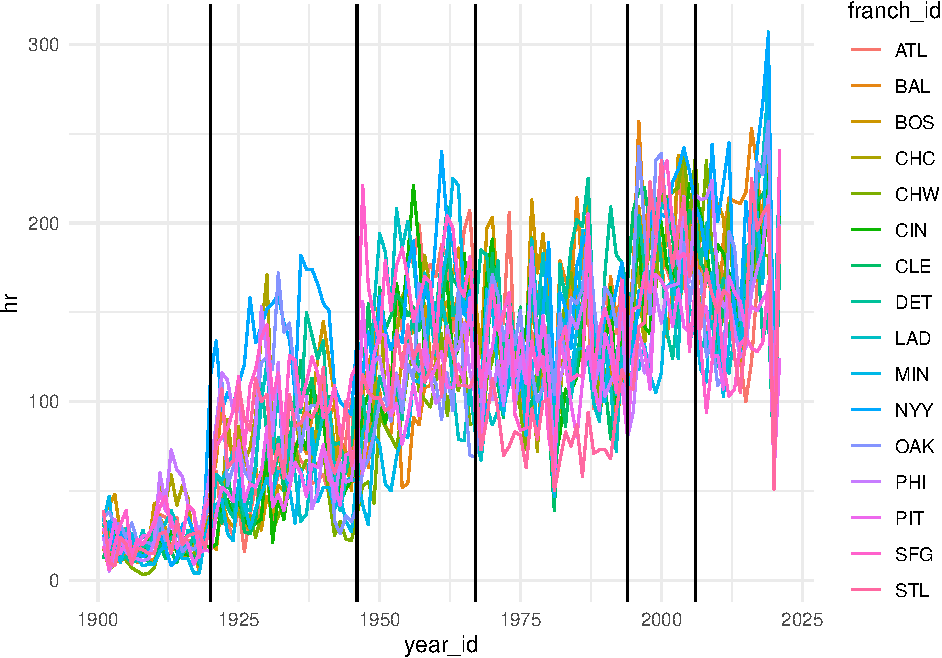
\includegraphics{paper_files/figure-latex/unnamed-chunk-1-1} \end{center}

\hypertarget{results-1}{%
\subsection{Results}\label{results-1}}

\begin{longtable}[]{@{}lrr@{}}
\toprule()
franch\_id & threshold & years \\
\midrule()
\endhead
NYY & 4.801818 & 1918 \\
BOS & 4.427752 & 1917 \\
BOS & 4.427752 & 1929 \\
BOS & 4.427752 & 1948 \\
BOS & 4.427752 & 1994 \\
LAD & 4.776867 & 1919 \\
LAD & 4.776867 & 1955 \\
ATL & 5.393778 & 1918 \\
ATL & 5.393778 & 1949 \\
CHW & 4.326192 & 1918 \\
CHC & 4.277577 & 1919 \\
CHC & 4.277577 & 1940 \\
CIN & 4.249476 & 1929 \\
CIN & 4.249476 & 1952 \\
CLE & 4.405339 & 1920 \\
CLE & 4.405339 & 1939 \\
DET & 3.926054 & 1927 \\
DET & 3.926054 & 1940 \\
BAL & 4.641706 & 1919 \\
BAL & 4.641706 & 1942 \\
SFG & 4.319634 & 1919 \\
SFG & 4.319634 & 1937 \\
OAK & 3.819294 & 1920 \\
OAK & 3.819294 & 1936 \\
OAK & 3.819294 & 1951 \\
PHI & 4.123104 & 1918 \\
PHI & 4.123104 & 1937 \\
PIT & 4.175793 & 1920 \\
PIT & 4.175793 & 1946 \\
STL & 5.444239 & 1919 \\
STL & 5.444239 & 1941 \\
MIN & 4.498666 & 1919 \\
MIN & 4.498666 & 1942 \\
\bottomrule()
\end{longtable}

NYY 1918: Babe Ruth got to the Yankees in 1920. And starting in 1919
they had exactly one losing seasons between 1919 and 1965.\\
BOS 1917, 1929, 1948, 1994: Their last world series win in the 1900s was
in 1918.\\
I don't know 1929. 1948 there was a big jump in runs?\\
1994: Strike year.

LAD: 1919, 1955

ATL 1918 1949

CHW: 1919: Blaack Sox Scandal

CHC: 1919 1940 1940: War.

Cin: 1929 1952

CLE 1920 1939 Cleveland won the world series in 1920. Major change in
offensive output.

DET 1927 1940

BAL 1919 1942

SFG 1919 1937

OAK 1920 1936 1951

PHI 1918 1937

PIT 1920 1946

STL 1919 1941

MIN 1919 1942

Pearl Harbor was 1941. So US was in war in 1942.

\hypertarget{acknowledgements}{%
\section*{Acknowledgements}\label{acknowledgements}}
\addcontentsline{toc}{section}{Acknowledgements}

We thank Michael Lopez for suggesting we do ``something with change
point analysis''.

\hypertarget{supplementary-material}{%
\section*{Supplementary Material}\label{supplementary-material}}
\addcontentsline{toc}{section}{Supplementary Material}

All code for reproducing the analyses in this paper is publicly
available at \url{https://github.com/menawhalen/baseball_cpt}

\hypertarget{references}{%
\section*{References}\label{references}}
\addcontentsline{toc}{section}{References}

\hypertarget{refs}{}
\begin{CSLReferences}{1}{0}
\leavevmode\vadjust pre{\hypertarget{ref-Cho2016}{}}%
Cho, H. 2016. {``Change-Point Detection in Panel Data via Double CUSUM
Statistic.''} \emph{Electronic Journal of Statistics} 10: 2000--2038.

\leavevmode\vadjust pre{\hypertarget{ref-hdbinseg}{}}%
Cho, Haeran, and Piotr Fryzlewicz. 2018. \emph{Hdbinseg: Change-Point
Analysis of High-Dimensional Time Series via Binary Segmentation}.
\url{https://CRAN.R-project.org/package=hdbinseg}.

\leavevmode\vadjust pre{\hypertarget{ref-ChoFryzlewwicz2014}{}}%
Cho, H., and P. Fryzlewicz. 2014. {``Multiple-Change-Point Detection for
High Dimensional Time Series via Sparsified Binary Segmentation.''}
\emph{JRSSB} 77: 475--507.

\leavevmode\vadjust pre{\hypertarget{ref-FortLee2007}{}}%
Fort, and Lee. 2007. {``Structural Change, Competitive Balance, and the
Rest of the Major Leagues.''} \emph{Economic Inquiry} 45 (3): 519--32.

\leavevmode\vadjust pre{\hypertarget{ref-Groothius2017}{}}%
Groothius, Peter A., Kurt W. Rotthoff, and Mark C. Strazicich. 2017.
{``Structural Breaks in the Game: The Case of Major League Baseball.''}
\emph{Journal of Sports Economics} 18 (6): 622--37.

\leavevmode\vadjust pre{\hypertarget{ref-PalaciosHuerta2004}{}}%
I., Palacios-Huerta. 2004. {``Structural Changes During a Century of the
World's Most Popular Sport.''} \emph{Statistical Methods and
Applications} 12: 241--58.

\leavevmode\vadjust pre{\hypertarget{ref-LeeandStrazicich2003}{}}%
Lee, J., and M. Strazicich. n.d. {``Minimum Lagrange Multiplier Unit
Root Test with Two Structural Breaks.''} \emph{The Review of Economics
and Statistics}, no. 4: 1082--89.

\leavevmode\vadjust pre{\hypertarget{ref-LeeFort2008}{}}%
Lee, Y. H., and R. Fort. 2008. {``Attendance and the
Uncertainty-of-Outcome Hypothesis in Baseball.''} \emph{Review of
Industrial Organization} 33 (4): 281--95.

\leavevmode\vadjust pre{\hypertarget{ref-LeeFort2005}{}}%
Lee, and Fort. 2005. {``Structural Change in MLB Competitive Balance:
The Depression, Team Location, and Integration.''} \emph{Economic
Inquiry} 43 (1): 158--69.

\leavevmode\vadjust pre{\hypertarget{ref-MillsFort2018}{}}%
Mills, Brian M., and Rodney Fort. 2018. {``Team-Level Time Series
Analysis in MLB, the NBA, and the NHL: Attendance and Outcome
Uncertainty.''} \emph{Journal of Sports Economics} 19 (7): 911--33.
\url{https://doi.org/10.1177/1527002517690787}.

\leavevmode\vadjust pre{\hypertarget{ref-MillsSalaga2015}{}}%
Mills, Brian M., and Steven Salaga. 2015. {``Historical Time Series
Perspectives on Competitive Balance in NCAA Division i Basketball.''}
\emph{Journal of Sports Economics} 16 (6): 614--46.
\url{https://doi.org/10.1177/1527002515580925}.

\leavevmode\vadjust pre{\hypertarget{ref-MillsFort2014}{}}%
MILLS, BRIAN, and RODNEY FORT. 2014. {``LEAGUE-LEVEL ATTENDANCE AND
OUTCOME UNCERTAINTY IN u.s. PRO SPORTS LEAGUES.''} \emph{Economic
Inquiry} 52 (1): 205--18.
https://doi.org/\url{https://doi.org/10.1111/ecin.12037}.

\leavevmode\vadjust pre{\hypertarget{ref-Noll1988}{}}%
Noll, R. G. 1988. {``Professional Basketball.''} \emph{Stanford
University Studies in Industrial Economics}, no. 144.

\leavevmode\vadjust pre{\hypertarget{ref-BBHOF1869}{}}%
Rothenberg, Matt. n.d. \emph{PRO BASEBALL BEGAN IN CINCINNATI IN 1869}.
\url{https://baseballhall.org/discover/pro-baseball-began-in-cincinnati-in-1869\#:~:text=The\%20Cincinnati\%20Red\%20Stockings\%20made,professional\%20baseball\%20club\%20in\%201869.}

\leavevmode\vadjust pre{\hypertarget{ref-SalagaFort2017}{}}%
Salaga, S., and R. Fort. 2017. {``Structural Change in Competitive
Balance in Big-Time College Football.''} \emph{Review of Industrial
Organization} 50: 27--41.

\leavevmode\vadjust pre{\hypertarget{ref-Scully1989}{}}%
Scully, G. W. 1989. \emph{The Business of Major League Baseball}.
University of Chicago Press.

\leavevmode\vadjust pre{\hypertarget{ref-Woltring2018}{}}%
Woltring, Rost, M., and C. Jubenville. 2018. {``Examining Perceptions of
Baseball's Eras: A Statistical Comparison.''} \emph{The Sport Journal}.
\url{https://thesportjournal.org/article/examining-perceptions-of-baseballs-eras/}.

\end{CSLReferences}

\end{document}
